\documentclass[tikz,border=5pt]{standalone}
\usepackage{pgfplots}
\pgfplotsset{compat=1.18}

\definecolor{corba}{HTML}{365FB3}

\begin{document}
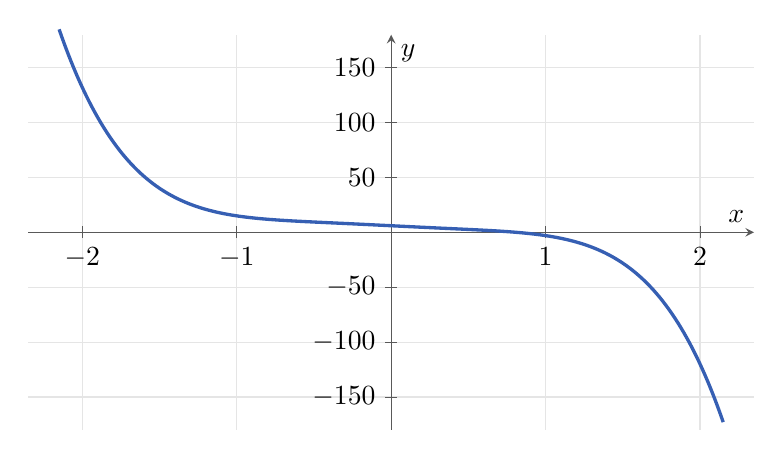
\begin{tikzpicture}
  \begin{axis}[
    width=10.8cm,
    height=6.6cm,
    axis lines=middle,
    xmin=-2.35,
    xmax=2.35,
    ymin=-180,
    ymax=180,
    xlabel={$x$},
    ylabel={$y$},
    xtick={-2,-1,1,2},
    ytick={-150,-100,-50,50,100,150},
    axis line style={black!65},
    tick style={black!65},
    grid=major,
    grid style={black!10},
    clip=false,
  ]
    \addplot[corba, very thick, domain=-2.15:2.15, samples=220]
      {-4*x^5+2*x^3-7*x+6};

  \end{axis}
\end{tikzpicture}
\end{document}
